%----------------------------------------------------------------------------
\appendix
%----------------------------------------------------------------------------
\chapter*{\fuggelek}\addcontentsline{toc}{chapter}{\fuggelek}
\setcounter{chapter}{\appendixnumber}
%\setcounter{equation}{0} % a fofejezet-szamlalo az angol ABC 6. betuje (F) lesz
\numberwithin{equation}{section}
\numberwithin{figure}{section}
\numberwithin{lstlisting}{section}
%\numberwithin{tabular}{section}

%----------------------------------------------------------------------------
\section{A more detailed metamodel for program ASGs}
%----------------------------------------------------------------------------

This metamodel fragment in \autoref{fig:example-extended-mm} contains all types required for the example instance model in \autoref{fig:example-instancemodel-handdrawn}.

\begin{figure}[!htp]
	\centering
	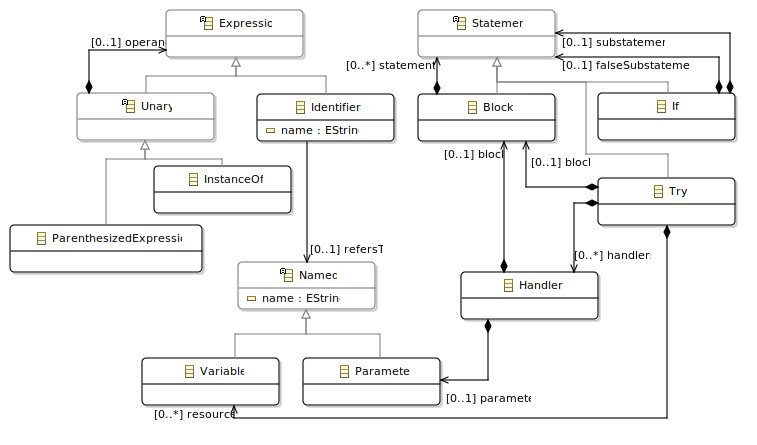
\includegraphics[width=\textwidth]{figures/pdfs/example-metamodel-extended-edited.pdf}
	\caption[~A more detailed EMF metamodel fragment for ASGs]{A more detailed EMF metamodel fragment for ASGs}
	\label{fig:example-extended-mm}
\end{figure}



%----------------------------------------------------------------------------
\clearpage\section{Detailed measurement results for code anti-patterns}
%----------------------------------------------------------------------------
\label{appendix:csmr-results}

Numeric output of the measurement process on the source code examples by phases is displayed in \autoref{tab:qwicap}, \autoref{tab:frinika}, and \autoref{tab:hibernate}.


%\clearpage
% latex table generated in R 3.2.2 by xtable 1.8-0 package
% Sun Dec 13 02:05:38 2015
\begin{table}[!htb]
	\centering
	\begin{tabular}{rllrrrr}
		\hline
		& Case & Tool & Read & \shortstack{\\Create\\engine} & \shortstack{Calculate\\search plan} & Check \\ 
		\hline \hline
		1 & Catch & Incremental & 0.082 & 0.097 & N/A & 0.0002 \\ 
		2 & Catch & Parallel & 0.092 & 0.032 & 0.008 & 0.0000 \\ 
		3 & Catch & Sequential & 0.064 & 0.067 & 0.010 & 0.0001 \\ 
		\hline
		4 & Constant compare & Incremental & 0.076 & 0.099 & N/A & 0.0002 \\ 
		5 & Constant compare & Parallel & 0.081 & 0.025 & 0.025 & 0.0014 \\ 
		6 & Constant compare & Sequential & 0.080 & 0.037 & 0.023 & 0.0007 \\ 
		\hline
		7 & No default switch & Incremental & 0.077 & 0.091 & N/A & 0.0001 \\ 
		8 & No default switch & Parallel & 0.082 & 0.026 & 0.001 & 0.0004 \\ 
		9 & No default switch & Sequential & 0.085 & 0.038 & 0.001 & 0.0002 \\ 
		\hline
		10 & Unused parameter & Incremental & 0.082 & 0.416 & N/A & 0.0013 \\ 
		11 & Unused parameter & Parallel & 0.092 & 0.126 & 0.086 & 0.0120 \\ 
		12 & Unused parameter & Sequential & 0.084 & 0.106 & 0.144 & 0.0063 \\ 
		\hline
	\end{tabular}
	\caption{Measurement results for Qwicap (in seconds)} 
	\label{tab:qwicap}
\end{table}

%\vspace{-10pt}
% latex table generated in R 3.2.2 by xtable 1.8-0 package
% Sun Dec 13 02:04:41 2015
\begin{table}[!htb]
	\centering
	\begin{tabular}{rllrrrr}
		\hline
		& Case & Tool & Read & \shortstack{\\Create\\engine} & \shortstack{Calculate\\search plan} & Check \\ 
		\hline \hline
		1 & Catch & Incremental & 2.535 & 1.813 & N/A & 0.0017 \\ 
		2 & Catch & Parallel & 2.575 & 0.855 & 0.406 & 0.0008 \\ 
		3 & Catch & Sequential & 2.512 & 0.842 & 0.400 & 0.0009 \\ 
		\hline
		4 & Constant compare & Incremental & 2.448 & 1.906 & N/A & 0.0014 \\ 
		5 & Constant compare & Parallel & 2.529 & 0.837 & 0.685 & 0.0052 \\ 
		6 & Constant compare & Sequential & 2.385 & 0.867 & 0.575 & 0.0081 \\
		\hline 
		7 & No default switch & Incremental & 2.535 & 1.628 & N/A & 0.0009 \\ 
		8 & No default switch & Parallel & 2.485 & 0.851 & 0.001 & 0.0007 \\ 
		9 & No default switch & Sequential & 2.395 & 0.840 & 0.001 & 0.0005 \\ 
		\hline
		10 & Unused parameter & Incremental & 2.458 & 3.105 & N/A & 0.0024 \\ 
		11 & Unused parameter & Parallel & 2.529 & 0.989 & 2.350 & 0.0711 \\ 
		12 & Unused parameter & Sequential & 2.406 & 0.912 & 2.283 & 0.0757 \\ 
		\hline
	\end{tabular}
	\caption{Measurement results for Frinika (in seconds)} 
	\label{tab:frinika}
\end{table}

%\vspace{-10pt}

% latex table generated in R 3.2.2 by xtable 1.8-0 package
% Sun Dec 13 01:46:46 2015
\begin{table}[!htpb]
	\centering
	\begin{tabular}{rllrrrr}
		\hline
		& Case & Tool & Read & \shortstack{\\Create\\engine} & \shortstack{Calculate\\search plan} & Check \\ 
		\hline \hline
		1 & Catch & Incremental & 17.858 & 10.588 & N/A & 0.0002 \\ 
		2 & Catch & Parallel & 16.671 & 4.925 & 2.698 & 0.0018 \\ 
		3 & Catch & Sequential & 16.377 & 4.758 & 2.647 & 0.0020 \\ 
		\hline
		4 & Constant compare & Incremental & 16.854 & 11.408 & N/A & 0.0007 \\ 
		5 & Constant compare & Parallel & 16.887 & 5.019 & 4.570 & 0.1888 \\ 
		6 & Constant compare & Sequential & 17.903 & 5.101 & 7.730 & 0.0588 \\ 
		\hline
		7 & No default switch & Incremental & 17.648 & 9.166 & N/A & 0.0002 \\ 
		8 & No default switch & Parallel & 16.620 & 4.683 & 0.001 & 0.0007 \\ 
		9 & No default switch & Sequential & 16.987 & 4.888 & 0.001 & 0.0003 \\ 
		\hline
		10 & Unused parameter & Incremental & 16.748 & 12.785 & N/A & 0.0008 \\ 
		11 & Unused parameter & Parallel & 16.776 & 4.702 & 9.959 & 0.2326 \\ 
		12 & Unused parameter & Sequential & 15.965 & 4.939 & 10.557 & 0.2632 \\ 
		\hline
	\end{tabular}
	\caption{Measurement results for Hibernate (in seconds)} 
	\label{tab:hibernate}
\end{table}

%----------------------------------------------------------------------------


\section{Detailed measurement results for Train Benchmark}
%----------------------------------------------------------------------------
\label{appendix:trainbenchmark-results}
\begin{minipage}{1.0\textwidth}
	
	Diagrams output by the Train Benchmark framework displaying the times needed for the different measurement phases by model sizes. Results for the Read and Crete engine phase is included in \autoref{fig:tb-measurements-read} and in \autoref{fig:tb-measurements-engine} below. Detailed measurement data is added in \autoref{tab:tb-inc}, \autoref{tab:tb-seq}, and in \autoref{tab:tb-par}.
	
	\centering
	\includegraphics[width=\linewidth]{pdfs/Batch-Read-phase.pdf}
	\vspace{-35pt}
	\captionof{figure}[~Train Benchmark -- Read phase]{Train Benchmark -- Read phase}
	\vspace{10pt}
	\label{fig:tb-measurements-read}
	
	\includegraphics[width=\linewidth]{pdfs/Batch-Create-engine-phase.pdf}
	\vspace{-35pt}
	\captionof{figure}[~Train Benchmark -- Create engine phase]{Train Benchmark -- Create engine phase}
	\vspace{15pt}
	
	\label{fig:tb-measurements-engine}
\end{minipage}

% latex table generated in R 3.2.2 by xtable 1.8-0 package
% Tue Dec 15 23:10:24 2015
\begin{table}[H]
	\centering
	\begin{tabular}{rlrrrrr}
		\hline
		& Case & \shortstack{Model\\scale}  & \shortstack{Calculate\\search plan} & Check & \shortstack{\\Create\\engine} & Read\\ 
		 
		\hline \hline
		1 & ConnectedSegments & 1 & N/A & 0.005 & 0.343 & 0.6160 \\ 
		2 & ConnectedSegments & 2 & N/A & 0.005 & 0.406 & 0.6973 \\ 
		3 & ConnectedSegments & 4 & N/A & 0.006 & 0.561 & 0.8009 \\ 
		4 & ConnectedSegments & 8 & N/A & 0.005 & 1.119 & 1.3233 \\ 
		5 & ConnectedSegments & 16 & N/A & 0.005 & 1.289 & 1.5371 \\ 
		6 & ConnectedSegments & 32 & N/A & 0.006 & 2.402 & 1.6769 \\ 
		7 & ConnectedSegments & 64 & N/A & 0.008 & 4.095 & 2.1386 \\ 
		8 & ConnectedSegments & 128 &  N/A& 0.009 & 5.975 & 2.7748 \\ 
		9 & ConnectedSegments & 256 &  N/A& 0.010 & 15.595 & 4.4905 \\ 
		10 & ConnectedSegments & 512 & N/A & 0.020 & 27.702 & 7.5964 \\ 
		11 & ConnectedSegments & 1024 &N/A  & 0.030 & 77.361 & 14.6564 \\ 
		11 & ConnectedSegments & 2048 & N/A  & - & - & - \\ 
		\hline
		12 & RouteSensor & 1 & N/A & 0.004 & 0.284 & 0.6573 \\ 
		13 & RouteSensor & 2 & N/A & 0.004 & 0.299 & 0.7124 \\ 
		14 & RouteSensor & 4 & N/A & 0.004 & 0.360 & 0.8038 \\ 
		15 & RouteSensor & 8 & N/A & 0.004 & 0.583 & 1.0638 \\ 
		16 & RouteSensor & 16 &N/A  & 0.004 & 0.832 & 1.1981 \\ 
		17 & RouteSensor & 32 &N/A  & 0.004 & 1.192 & 1.5331 \\ 
		18 & RouteSensor & 64 &N/A  & 0.006 & 1.583 & 1.8914 \\ 
		19 & RouteSensor & 128 & N/A & 0.005 & 2.416 & 2.7768 \\ 
		20 & RouteSensor & 256 & N/A & 0.006 & 4.279 & 4.6098 \\ 
		21 & RouteSensor & 512 & N/A & 0.007 & 7.726 & 7.7939 \\ 
		22 & RouteSensor & 1024 &N/A  & 0.009 & 14.953 & 14.2515 \\ 
		23 & RouteSensor & 2048 &N/A  & 0.017 & 29.599 & 31.1415 \\ 
		\hline
		24 & SemaphoreNeighbor & 1 &  N/A& 0.004 & 0.302 & 0.6278 \\ 
		25 & SemaphoreNeighbor & 2 &  N/A& 0.005 & 0.346 & 0.7314 \\ 
		26 & SemaphoreNeighbor & 4 &  N/A& 0.003 & 0.564 & 0.9943 \\ 
		27 & SemaphoreNeighbor & 8 &  N/A& 0.004 & 0.644 & 1.2172 \\ 
		28 & SemaphoreNeighbor & 16 & N/A & 0.005 & 0.920 & 1.2461 \\ 
		29 & SemaphoreNeighbor & 32 & N/A & 0.004 & 1.516 & 1.5093 \\ 
		30 & SemaphoreNeighbor & 64 & N/A & 0.006 & 2.436 & 2.0862 \\ 
		31 & SemaphoreNeighbor & 128 &N/A  & 0.005 & 4.065 & 2.8686 \\ 
		32 & SemaphoreNeighbor & 256 &N/A  & 0.006 & 7.648 & 4.5046 \\ 
		33 & SemaphoreNeighbor & 512 &N/A  & 0.006 & 14.986 & 7.6752 \\ 
		34 & SemaphoreNeighbor & 1024 & N/A & 0.005 & 28.147 & 14.2688 \\ 
		35 & SemaphoreNeighbor & 2048 & N/A & 0.007 & 53.646 & 29.8475 \\ 
		\hline
		36 & SwitchSet & 1 & N/A & 0.004 & 0.298 & 0.6307 \\ 
		37 & SwitchSet & 2 & N/A & 0.004 & 0.299 & 0.7143 \\ 
		38 & SwitchSet & 4 & N/A & 0.004 & 0.413 & 0.9119 \\ 
		39 & SwitchSet & 8 & N/A & 0.004 & 0.500 & 1.1864 \\ 
		40 & SwitchSet & 16 &N/A  & 0.005 & 0.628 & 1.3747 \\ 
		41 & SwitchSet & 32 &N/A  & 0.004 & 1.075 & 1.5935 \\ 
		42 & SwitchSet & 64 &N/A  & 0.005 & 1.439 & 1.9664 \\ 
		43 & SwitchSet & 128 & N/A & 0.006 & 2.134 & 2.8516 \\ 
		44 & SwitchSet & 256 & N/A & 0.007 & 3.714 & 4.6632 \\ 
		45 & SwitchSet & 512 & N/A & 0.009 & 6.989 & 7.8651 \\ 
		46 & SwitchSet & 1024 &N/A  & 0.011 & 13.969 & 14.4903 \\ 
		47 & SwitchSet & 2048 &N/A  & 0.016 & 23.615 & 29.4733 \\ 
		\hline
	\end{tabular}
	\caption{Benchmark results for the incremental algorithm}
	\label{tab:tb-inc}
\end{table}


% latex table generated in R 3.2.2 by xtable 1.8-0 package
% Tue Dec 15 23:21:03 2015
\begin{table}[ht]
	\centering
	\begin{tabular}{rlrrrrr}
				\hline
		& Case & \shortstack{Model\\scale}  & \shortstack{Calculate\\search plan} & Check & \shortstack{\\Create\\engine} & Read\\ 
		\hline
		\hline
		48 & ConnectedSegments & 1 & 0.047 & 0.074 & 0.175 & 0.5428 \\ 
		49 & ConnectedSegments & 2 & 0.043 & 0.037 & 0.160 & 0.6564 \\ 
		50 & ConnectedSegments & 4 & 0.081 & 0.050 & 0.210 & 1.4798 \\ 
		51 & ConnectedSegments & 8 & 0.262 & 0.086 & 0.289 & 0.9131 \\ 
		52 & ConnectedSegments & 16 & 0.396 & 0.128 & 0.348 & 1.1620 \\ 
		53 & ConnectedSegments & 32 & 1.202 & 0.276 & 0.763 & 1.3668 \\ 
		54 & ConnectedSegments & 64 & 2.496 & 0.240 & 1.026 & 1.8711 \\ 
		55 & ConnectedSegments & 128 & 5.115 & 0.341 & 1.423 & 2.6572 \\ 
		56 & ConnectedSegments & 256 & 10.875 & 0.458 & 2.678 & 4.0401 \\ 
		57 & ConnectedSegments & 512 & 14.811 & 1.289 & 4.648 & 7.9337 \\ 
		58 & ConnectedSegments & 1024 & 28.935 & 2.672 & 9.810 & 13.1614 \\ 
		59 & ConnectedSegments & 2048 & 81.477 & 21.778 & 16.030 & 27.3225 \\ 
		\hline
		60 & RouteSensor & 1 & 0.014 & 0.020 & 0.156 & 0.5635 \\ 
		61 & RouteSensor & 2 & 0.019 & 0.024 & 0.173 & 0.6561 \\ 
		62 & RouteSensor & 4 & 0.027 & 0.029 & 0.190 & 0.7796 \\ 
		63 & RouteSensor & 8 & 0.072 & 0.034 & 0.263 & 1.4431 \\ 
		64 & RouteSensor & 16 & 0.119 & 0.045 & 0.396 & 1.1981 \\ 
		65 & RouteSensor & 32 & 0.284 & 0.053 & 0.785 & 1.6905 \\ 
		66 & RouteSensor & 64 & 0.542 & 0.067 & 0.967 & 1.9556 \\ 
		67 & RouteSensor & 128 & 1.207 & 0.104 & 1.406 & 2.6108 \\ 
		68 & RouteSensor & 256 & 2.539 & 0.151 & 2.669 & 4.3887 \\ 
		69 & RouteSensor & 512 & 3.800 & 0.189 & 4.885 & 6.8383 \\ 
		70 & RouteSensor & 1024 & 7.025 & 0.285 & 9.403 & 11.9807 \\ 
		71 & RouteSensor & 2048 & 14.836 & 0.380 & 16.569 & 25.7272 \\ 
		\hline
		72 & SemaphoreNeighbor & 1 & 0.024 & 0.040 & 0.145 & 0.5200 \\ 
		73 & SemaphoreNeighbor & 2 & 0.041 & 0.052 & 0.176 & 0.5795 \\ 
		74 & SemaphoreNeighbor & 4 & 0.066 & 0.083 & 0.199 & 1.0330 \\ 
		75 & SemaphoreNeighbor & 8 & 0.103 & 0.050 & 0.268 & 1.2399 \\ 
		76 & SemaphoreNeighbor & 16 & 0.210 & 0.195 & 0.351 & 1.1655 \\ 
		77 & SemaphoreNeighbor & 32 & 0.702 & 0.231 & 0.646 & 1.6327 \\ 
		78 & SemaphoreNeighbor & 64 & 1.534 & 0.422 & 1.113 & 1.7387 \\ 
		79 & SemaphoreNeighbor & 128 & 2.776 & 0.123 & 1.400 & 2.4430 \\ 
		80 & SemaphoreNeighbor & 256 & 5.743 & 1.732 & 2.543 & 4.1405 \\ 
		81 & SemaphoreNeighbor & 512 & 7.488 & 0.250 & 4.615 & 7.1392 \\ 
		82 & SemaphoreNeighbor & 1024 & 15.876 & 1.702 & 9.112 & 12.2774 \\ 
		83 & SemaphoreNeighbor & 2048 & 52.981 & 0.665 & 17.138 & 26.8228 \\ 
		\hline
		84 & SwitchSet & 1 & 0.019 & 0.011 & 0.145 & 0.5297 \\ 
		85 & SwitchSet & 2 & 0.025 & 0.017 & 0.173 & 0.6714 \\ 
		86 & SwitchSet & 4 & 0.028 & 0.021 & 0.209 & 0.7397 \\ 
		87 & SwitchSet & 8 & 0.037 & 0.028 & 0.375 & 1.0071 \\ 
		88 & SwitchSet & 16 & 0.064 & 0.027 & 0.337 & 1.1823 \\ 
		89 & SwitchSet & 32 & 0.230 & 0.025 & 0.599 & 1.3891 \\ 
		90 & SwitchSet & 64 & 0.497 & 0.047 & 0.954 & 1.8049 \\ 
		91 & SwitchSet & 128 & 0.895 & 0.038 & 1.307 & 2.6413 \\ 
		92 & SwitchSet & 256 & 2.009 & 0.069 & 2.480 & 4.3071 \\ 
		93 & SwitchSet & 512 & 2.885 & 0.084 & 4.675 & 7.1133 \\ 
		94 & SwitchSet & 1024 & 6.073 & 0.131 & 9.606 & 12.4735 \\ 
		95 & SwitchSet & 2048 & 11.590 & 0.148 & 17.169 & 28.1495 \\ 
		\hline
	\end{tabular}
	\caption{Benchmark result for the sequential local search-based algorithm}
		\label{tab:tb-seq}
\end{table}


% latex table generated in R 3.2.2 by xtable 1.8-0 package
% Tue Dec 15 23:40:09 2015
\begin{table}[ht]
	\centering
	\begin{tabular}{rlrrrrr}
		\hline
		& Case & \shortstack{Model\\scale}  & \shortstack{Calculate\\search plan} & Check & \shortstack{\\Create\\engine} & Read\\ 
		\hline
		\hline
		96 & ConnectedSegments & 1 & 0.160 & 0.029 & 0.182 & 0.6048 \\ 
		97 & ConnectedSegments & 2 & 0.179 & 0.041 & 0.200 & 0.6937 \\ 
		98 & ConnectedSegments & 4 & 0.240 & 0.069 & 0.234 & 2.8547 \\ 
		99 & ConnectedSegments & 8 & 0.455 & 0.079 & 0.295 & 1.0115 \\ 
		100 & ConnectedSegments & 16 & 0.859 & 0.247 & 0.411 & 1.2394 \\ 
		101 & ConnectedSegments & 32 & 2.020 & 0.258 & 0.661 & 1.5176 \\ 
		102 & ConnectedSegments & 64 & 3.175 & 0.735 & 1.162 & 2.0864 \\ 
		103 & ConnectedSegments & 128 & 6.631 & 0.827 & 1.438 & 2.8166 \\ 
		104 & ConnectedSegments & 256 & 14.495 & 3.906 & 2.361 & 4.4578 \\ 
		105 & ConnectedSegments & 512 & 20.719 & 3.109 & 4.542 & 8.2206 \\ 
		106 & ConnectedSegments & 1024 & 39.900 & 6.585 & 9.425 & 14.7102 \\ 
		107 & ConnectedSegments & 2048 & 104.046 & 34.750 & 17.492 & 29.6772 \\
		\hline
		108 & RouteSensor & 1 & 0.092 & 0.006 & 0.165 & 0.6108 \\ 
		109 & RouteSensor & 2 & 0.104 & 0.009 & 0.180 & 0.6993 \\ 
		110 & RouteSensor & 4 & 0.147 & 0.014 & 0.225 & 0.8292 \\ 
		111 & RouteSensor & 8 & 0.265 & 0.023 & 0.302 & 1.0207 \\ 
		112 & RouteSensor & 16 & 0.471 & 0.034 & 0.567 & 1.3270 \\ 
		113 & RouteSensor & 32 & 0.795 & 0.060 & 0.708 & 1.5513 \\ 
		114 & RouteSensor & 64 & 1.398 & 0.067 & 1.019 & 1.9423 \\ 
		115 & RouteSensor & 128 & 2.529 & 0.102 & 1.655 & 2.9249 \\ 
		116 & RouteSensor & 256 & 5.121 & 0.174 & 2.583 & 4.7742 \\ 
		117 & RouteSensor & 512 & 10.334 & 0.227 & 4.330 & 7.7517 \\ 
		118 & RouteSensor & 1024 & 19.039 & 0.488 & 10.023 & 14.7573 \\ 
		119 & RouteSensor & 2048 & 38.614 & 0.525 & 17.730 & 30.2251 \\ 
		\hline
		120 & SemaphoreNeighbor & 1 & 0.138 & 0.036 & 0.181 & 0.6367 \\ 
		121 & SemaphoreNeighbor & 2 & 0.152 & 0.060 & 0.200 & 0.7069 \\ 
		122 & SemaphoreNeighbor & 4 & 0.206 & 0.100 & 0.221 & 0.8413 \\ 
		123 & SemaphoreNeighbor & 8 & 0.353 & 0.084 & 0.302 & 1.0385 \\ 
		124 & SemaphoreNeighbor & 16 & 0.663 & 0.133 & 0.395 & 1.2638 \\ 
		125 & SemaphoreNeighbor & 32 & 1.355 & 0.356 & 0.648 & 1.5020 \\ 
		126 & SemaphoreNeighbor & 64 & 1.993 & 0.287 & 1.254 & 2.0495 \\ 
		127 & SemaphoreNeighbor & 128 & 4.037 & 0.957 & 1.554 & 2.9425 \\ 
		128 & SemaphoreNeighbor & 256 & 8.168 & 0.994 & 2.621 & 4.6234 \\ 
		129 & SemaphoreNeighbor & 512 & 14.477 & 2.945 & 4.356 & 8.0286 \\ 
		130 & SemaphoreNeighbor & 1024 & 27.131 & 6.580 & 9.242 & 14.5130 \\ 
		131 & SemaphoreNeighbor & 2048 & 52.988 & 44.576 & 17.004 & 28.2886 \\ 
		\hline
		132 & SwitchSet & 1 & 0.105 & 0.004 & 0.165 & 0.6604 \\ 
		133 & SwitchSet & 2 & 0.113 & 0.005 & 0.183 & 0.6893 \\ 
		134 & SwitchSet & 4 & 0.151 & 0.009 & 0.222 & 0.9518 \\ 
		135 & SwitchSet & 8 & 0.232 & 0.010 & 0.309 & 1.1063 \\ 
		136 & SwitchSet & 16 & 0.354 & 0.014 & 0.408 & 1.3451 \\ 
		137 & SwitchSet & 32 & 0.736 & 0.025 & 0.718 & 1.6062 \\ 
		138 & SwitchSet & 64 & 1.044 & 0.033 & 1.211 & 2.0653 \\ 
		139 & SwitchSet & 128 & 2.188 & 0.056 & 1.622 & 2.8650 \\ 
		140 & SwitchSet & 256 & 5.262 & 0.093 & 2.735 & 4.7560 \\ 
		141 & SwitchSet & 512 & 9.661 & 0.132 & 4.624 & 7.6547 \\ 
		142 & SwitchSet & 1024 & 18.099 & 0.142 & 9.202 & 13.4744 \\ 
		143 & SwitchSet & 2048 & 34.605 & 0.262 & 17.445 & 29.0464 \\ 
		\hline
	\end{tabular}
	\caption{Benchmark result for the parallel local search-based algorithm}
	\label{tab:tb-par}		
\end{table}